%%% Local Variables:
%%% mode: latex
%%% TeX-master: t
%%% End:

\chapter{引言}
\label{cha:intro}
%引出问题。

\section{中断}
\label{sec:intr}
中断(Interrupt)是指处理器接收到特殊信号,提示某个事件发生,应当采取
对应措施的情况。发出这样的信号的行为被称作中断请求(Interrupt Request,
IRQ)。这个信号可以是来自外围硬件的异步信号,也可以是由运行在处理器上的
软件发出同步信号。前者被称为硬件中断(Hardware Interrupt),后者则被
称为软件中断(Software Interrupt,常简称为软中断)。

处理器在接收到中断信号以后,通常会保存当前的执行状态,该执行状态被称为上
下文(Context)。上下文的内容视各个硬件平台的不同而有所区别,但是大多包
含程序计数器(Program Counter,PC)和程序状态字以及部分通用计算寄存器。
之后,处理器会根据中断向量表的指示跳转到指定代码片段,即当前中断的处理程
序。在执行完中断处理程序之后,处理器会重新加载之前保存的上下文,继续执行
之前被打断的程序。进入中断和退出中断都包含了将保存当前上下文,载入新的上
下文的操作。此类操作被称作为上下文切换(Context Switch)。\footnote{严
格意义上的上下文切换并不要求保存一个完好的上下文,载入另一个完好的上下文,
实际情况中经常发生载入的上下文只有部分内容有意义的情况。或者对原有上下文
并未做出妥善保存即另行载入,相当于舍弃了当前上下文。这在处理器响应中断时
尤其多见。}

人们引入中断是为了提高计算机系统的性能。如果没有中断,处理器在接受外部硬
件通信时只能采取轮询方式。例如,处理器向某硬件发出某指令并需求其回复时,
只能采取繁忙等待(Busy-waiting)模式,这样就会浪费许多处理器周期。即使
在软件层面运用多线程技术进行优化,此类轮询操作依然是性能的损失。在引入中
断之后,处理器就可以专注于当前任务,并且可以在需要时候与外部硬件通信,从
而大幅提高运行效率。\footnote{处理器检查中断的原理其实也类似于一个轮询
操作。每个周期,处理器会检查特定的寄存器的某些位来判断是否有中断需要处理。
只不过这个处理相比于外部硬件通信快速得多。}后来被用于CPU外部与内部紧急事
件的处理、机器故障的处理、时间控制等多个方面,并产生通过软件方式进入中断
处理(软中断)的概念。在处理中断时几乎必然会触发两次切换上下文的操作,该
操作会涉及内存访问,因此其耗时在中断处理程序本身比较短的时候也不可忽略。
过于频繁的中断触发也会在一定程度降低系统的性能。

中断系统在硬件实现上可以是一个包含控制线路的独立系统,也可以被集成进存储
器子系统中。对于前者,在IBM个人机上,广泛使用可编程中断控制器(Programmable 
Interrupt Controller,PIC)来负责中断响应和处理。PIC被连接在若干中
断请求设备和处理器的中断引脚之间,从而实现对处理器中断请求线路(多为一针
或两针)的复用。作为另一种中断实现的形式,即存储器子系统实现方式,可以将
中断端口映射到存储器的地址空间,这样对特定存储器地址的访问实际上是中断请
求。一般桌面领域的PC机中,中断控制器一般是集成在处理器内部,\footnote{
例如\intel{}推出的8086系列处理器中,集成了\intel{} 8259系列中断控制器。}
而在嵌入式领域,很多厂商推出的微控制器实现了外置的中断控制器。\footnote{
例如意法半导体(STMicroelectronics)推出的STM32F4系列微控制器中,在ARM
的CPU外提供了中断控制器。}

\subsection{操作系统中的中断}
\label{subsec:intr_OS}
在实际应用中,中断的行为并不一直忠实地遵从其硬件实现,操作系统可以在一定
程度上改变中断的行为。在嵌入式操作系统中,出于实时性的考虑,一个中断的运
行时间不应该过长,但是许多中断需要实现的逻辑功能却比较复杂。因此一个通用
的解决方案就是在操作系统中将中断分成两段,前一段在中断触发时立即执行,后
一段则延后执行。后一段代码的执行优先级较低,因此有可能被其他低优先级中断
甚至是普通代码抢先执行。这样,在编写中断代码的时候,将需要立即执行不容延
迟同时运行时间较短的代码放在第一段,其他的对延时不敏感,或者任务繁重,或
者需要和其他线程进行同步交互的代码放在第二段,就能在满足实时性要求的前提
下完成该中断。eCos等许多操作系统尽管实现方式各异,采用的都是分段中断的模
式。\cite{ecos}图~\ref{fig:intr_exec} 和图~\ref{fig:ecos_intr_exec} 
分别展示了两种中断的执行流。

\begin{figure}[H]
	\centering
	\subcaptionbox{普通中断的执行流\label{fig:intr_exec}}
	{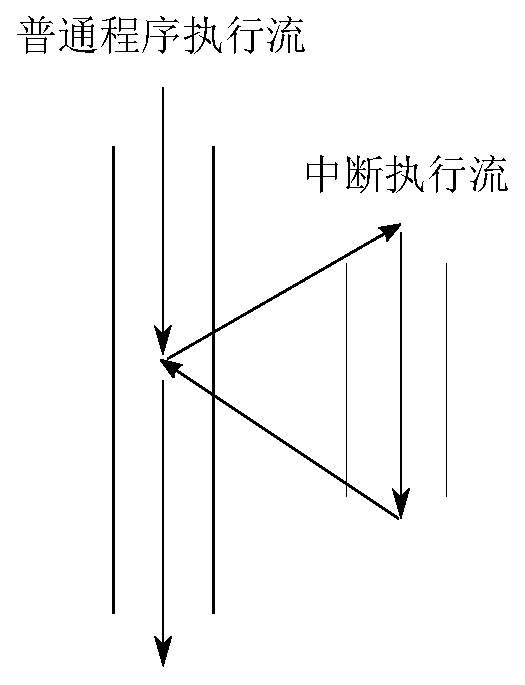
\includegraphics[width=0.35\textwidth]{interrupt_exec_model}}
	\hspace{4em}%
	\subcaptionbox{分段中断的执行流\label{fig:ecos_intr_exec}}
	{\includegraphics[width=0.35\textwidth]{ecos_interrupt_model}}
	\caption{不同的中断执行流}
	\label{fig:two_intr_exec}
\end{figure}

\section{程序的正确性}
\label{sec:correctness}
人们通常关心程序的许多性质。我们常说一个程序是否正确,其实涵盖了很多方面。

程序正确性,从狭义上来说,是指一段代码实现的功能是否如预期。这个要求并没
有看上去那么简单。程序不仅在接受各种合法输入之后需要给出预期的输出,在接
受非法输入之后也应该能判断出输入非法,并作出相应的处理措施。

从广义上来说,程序正确性还包含了其在指定环境下运行的正确性。现在的程序很
少是完全孤立运行。大部分程序运行在操作系统中,需要与其他程序共享CPU,内
存,硬盘,网络等资源。那么,程序的正确性就包含了该程序在共享资源的条件下
依然能保持上述狭义的正确性质。对多线程程序的研究就是着眼于多个线程在共享
CPU的条件下能否保证其功能的正确,尤其是当线程间共享的资源不仅仅是CPU,
还有内存中的变量,共同的文件或网络链接等资源时,情况将变得更加复杂。即使
在单线程的运行环境中,程序还会受到中断的干扰\footnote{上述的多线程的环
境下,通常也是有中断存在的。多线程的时间片轮转模式就完全依赖时钟中断。只
不过由于多线程的运行环境已经十分复杂,许多研究就忽略了中断的参与以简化问
题。}除了时钟中断以外的其他中断相比多线程环境,行为的随机性更高,一旦出现
问题,想要完全重现问题场景更为困难,研究起来更加困难。

由于外部环境的参与,一些原本不属于正确性的性质也会对程序的正确运行产生影
响。举个例子,程序的运行时间在大多数情况,本与程序是否正确没有关系,从软
件工程的需求分析角度来说,运行时间,或者说效率只能算作程序的非功能需求。
一段程序运行时间长短似乎不会影响到程序运行的结果。然而,事实并非总是如此。

当程序的运行时间影响到共享资源的占用,而共享资源又对程序的功能正确性造成
影响的时候,程序的运行时间就会成为程序正确性的内涵之一。这在一些十分接近
硬件底层的程序中,体现得尤为明显。举个简单的例子,一个简单的Clinet-Server
(CS)架构,一个客户端和一个服务器。客户端给服务器发送一个请求,经过一段
时间服务器返回结果,客户端继续一段逻辑。在网络编程中,考虑到网络环境的不
稳定性,程序员通常会设置等待超时,即当一定时间后得不到网络另一端的响应,
就认为此次请求失效,接下来就进行例如重发等措施。在这个场景下,服务器接受
请求返回应答的程序的运行时间就会成为影响客户端程序正确性的因素。在极端情
况下,服务器端程序的运行时间过长,客户端一直无法在超时限制之前得到响应,
那么客户端的正常逻辑就永远无法进行下去。

在实时软件系统中,由于实时性要求非常高,大部分程序的运行时间都是其正确性
的关键内容。在大部分实时软件系统中,中断多且与整个软件系统的功能息息相关。
的正确性就显得尤为重要。中断本身的难以预测,中断之间的相互作用又
使得中断的时间性质验证相对困难。

\section{程序的验证技术}
\label{sec:verification}
编程技术发展至今,软件的验证技术已经日趋成熟。根据是否运行程序,我们可以
将验证技术分为动态验证技术和静态验证技术两大类。

\subsection{动态验证技术}
\label{subsec:dynamic}
动态验证即我们通常所谓的测试。根据测试范围的不同,我们可将测试分为三类。
\cite{SWEBOK}
\begin{itemize}
	\item 小范围测试:测试一个函数或一个类(单元测试)
	\item 大范围测试:测试一组类,例如
	\begin{enumerate}[(1)]
		\item 模块测试(测试一个模块)
		\item 集成测试(测试多个模块)
		\item 系统测试(测试整个系统)
	\end{enumerate}
	\item 验收测试:验证软件是否满足需求的正式测试
	\begin{enumerate}[(1)]
		\item 功能测试
		\item 非功能测试(性能测试,压力测试等)
	\end{enumerate}		
\end{itemize}
测试一直时软件工程中十分重要也是最常规的验证的手段。在大多数场合,软件测
试成本低,效果显著。在成熟的软件公司或软件开发团队中,都有专门从事测试的
部门或人员。

\subsection{静态验证技术}
\label{subsec:static}
静态验证指在不运行程序的前提下,对程序进行的验证。有些程序的测试成本太高,
或者测试用例无法覆盖正常运行时的很多情形,即当我们无法测试程序,或者测试
结果局限性太严重时,我们转向静态验证。静态验证的技术发展多年,已经有了很
多相对成熟的方案。例如:
\begin{itemize}
	\item 代码规范检查
	\item 反例检测
	\item 形式化验证
	\begin{enumerate}[(1)]
		\item 模型检测
		\item 定理证明
	\end{enumerate}	
\end{itemize}

在静态分析技术中,形式化验证利用形式化方法对程序性质进行验证,由于其在理
论上的可靠性受到学术界密切关注。常规的测试很难甚至不可能在可以容忍的时间
内覆盖所有的可能情况,但是形式化验证技术则在理论上有给出一个完全覆盖所有
可能的测试结果的可能。这就是形式化验证相比传统动态验证技术的最大优势。

%这一段加引用
在诸多形式化验证技术中,模型检测由于数学要求相对不高,自动化程度较高,工
具化较为容易,在学术界较为流行。定理证明作为另一个完全不同的分支,由于自
动化程度和工具化程度太低,大量工作需要人的手工参与,因此使用者相对较少,
应用数量较少。但是,这模型检测和定理证明在大规模项目上的应用都有限制。前
者受理论和计算机硬件的限制,状态空间爆炸这个问题一直无法根本解决。这也是
诸多学者一直在努力的方向之一。后者由于其理论依据中对高阶逻辑的支持,看似
可以在理论上解决空间爆炸的问题,但是由于目前定理证明主要还是靠人工参与推
理,面对大型项目,人工的推理几乎不可完成。理论上可以进行验证,但是成本过
于高昂,这也是工业界对形式化验证技术一直难以应用的主要原因。相比之下,传
统的测试技术,对项目敏感度没有形式化技术这么高,反而容易取得不错的结果。

然而,在一些领域,程序的正确性涉及到人身财产安全甚至国家安全,不完备的测
试几乎不可能满足正确性的验证要求。形式化验证看似很美好,但随着验证规模的
增长,成本也成指数级增长,这时一个折中的做法对验证对象进行一定的抽象,然
后再对抽象出的模型进行验证。通常,抽象之后的模型相比原程序在验证规模上会
缩小很多。如果能保证抽象过程对于待验证性质的保持,即针对待验证性质,程序
和抽象模型之间存在一个完好的精化关系,就可以对模型进行形式化验证。

\section{研究课题}
\label{sec:subject}
我的课题是基于Uppaal的中断实时性的分析和验证。课题来源于一个针对某嵌入
式平台的实时软件系统的验证项目。我希望利用时间自动机的理论分析中断的时间
性质,进而对某些性质给出肯定或否定的验证结论。

\subsection{Uppaal简介}
\label{subsec:Uppaal_intro}
%这一段加引用
UPPAAL是一个进行建模,仿真和验证实时系统的集成工具环境,由丹麦奥尔堡大
学的计算机科学基础研究中心(Basic Research in Computer Science, BRICS)和瑞典乌普萨拉大学信息技术系联合开发。它适合那些可以被建模为具有
有限的控制结构和实数值时钟,通过信道或共享变量通信的非确定性过程集合的系
统。典型的应用领域包括实时控制器和特定的实时性至关重要的通信协议。

\subsection{预期成果}
\label{subsec:expectation}
本课题预期有以下成果:
\begin{itemize}
	\item 在Uppaal中针对各类中断的时间自动机模型
	\item 针对某嵌入式平台的实时软件系统的中断的时间性质的验证
\end{itemize}

\section{论文结构}
\label{sec:structure}
本文第一章简要介绍我研究的课题以及相关背景。在第二章,本文将介绍一些有关
中断分析验证以及时间自动机的相关工作。在第三章,本文将描述对中断行为的分
析,中断模型的建立和利用时间自动机的分析过程。在第四章,本文将描述将本文
的理论模型应用某嵌入式平台的实施软件系统进行验证的实验过程以及实验结果。
在第五章,本文将对该课题工作进行总结。


